\documentclass[12pt]{extarticle}
\usepackage[english]{babel}
\usepackage{NotesTeX}
\usepackage{subfigure}
\usepackage{tikz}
\usetikzlibrary{arrows}
\usepackage{multirow}
\usepackage{listings}
\usepackage{extarrows}
\usepackage{parskip}
\usepackage{eurosym}
\usepackage{footmisc}

\graphicspath{{../output/}}
\collaborationImg{
\includegraphics[width=30mm]{../../pictures/UIO.png}}

\author{\Large Vetle Nevland, Vetle Vikenes \& Sigurd Sørlie Rustad}
\title{\Huge Machine Learning: Bra Tittel}
\affiliation{\large FYS-STK4155 – Applied Data Analysis and Machine Learning
\\Autumn 2021\\Department of Physics\\University of Oslo\\\\\today}
\begin{document}
\abstract{Coming soon!
}
\maketitle
\pagestyle{myplain}

\section{Introduction}

We will in no way answer all questions linked to the aforementioned methods. So that anyone can reproduce or continue our studies, we list all the code, results and instructions on running the code in our GitHub repository\footnote{\href{https://github.com/sigurdru/FYS-STK4155/tree/main/project2}{https://github.com/sigurdru/FYS-STK4155/tree/main/project3}}.

\section{Theory}
In the theory-section we aim to give a brief explanation of the main concepts and terminology used in this report. 

\subsection{The diffusion equation}

The full diffusion equation reads
\begin{equation}
\frac{\partial u(\mathbf{r}, t)}{\partial t} = \nabla \cdot \left[D(u, \mathbf{r})\nabla u(\mathbf{r}, t)\right],
\end{equation}
where $\mathbf{r}$ is a positional vector and $D(u,r)$ the collective diffusion coefficient. If $D(u,\mathbf{r}) = 1$ the equation simplifies to a linear differential equation
\begin{equation}
\frac{\partial u}{\partial t} = \nabla^2u(\mathbf{r}, t),
\end{equation}
or
\begin{equation}
\label{eq:diffusion_equation}
\left(\frac{\partial^2}{\partial x^2} + \frac{\partial^2}{\partial y^2} + \frac{\partial^2}{\partial z^2}\right) u(x,y,z,t) = \frac{\partial u(x,y,z,t)}{\partial t}
\end{equation}
in cartesian coordinates. In this report we are going to study a one dimensional rod of length $L=1$. I.e. we need the one dimensional diffusion equation
\begin{align}
\label{eq:diffusion_equation_1D}
\frac{\partial^2 u(x,t)}{\partial x^2} &= \frac{\partial u(x,t)}{\partial t},
\end{align}
with boundary conditions
\begin{align}
u(x,0) &= \sin(\pi x) \ \ 0\leq x\leq L,\\
u(0,t) &= 0 \ \ t\geq 0 \text{ and} \\
u(L,t) &= 0 \ \ t\geq 0.
\end{align}

\subsection{Analytical solution}
An analytical solution of the 1D diffusion equation can be dervied using the method of separation of variables.
\[ u(x,t) = X(x)T(t) \]
The solution is separated into a function $X$ only depending on the independent variable $x$, and a function $T$ only depending on the independent variable $t$. Equation \ref{eq:diffusion_equation_1D} can then be rewritten as

\begin{align*}
	\frac{\partial^2 X(x)T(t)}{\partial x^2} &= \frac{\partial X(x)T(t)}{\partial t} \\
	T(t)\frac{\partial^2 X(x)}{\partial x^2} &= X(x)\frac{\partial T(t)}{\partial t} \\
	\frac{1}{X}\frac{\partial^2 X(x)}{\partial x^2} &= \frac{1}{T}\frac{\partial T(t)}{\partial t}
\end{align*}

The core of the method now becomes clear. The independent variables are separated and put on either side of the equation. Because $x$ and $t$ are independent we may fix one of them, say $x$, while letting the other ($t$) vary. The left side of the equation is thus constant, and since we have equality the expression on the right side must equal the same constant, for arbitrary $t$. Therefore, we can set the left side and right side equal to a constant $-k^2$. The reason for defining a negative constant is to prevent a growing solution, which will be clear on the derivation.

\[ \frac{1}{X}\frac{\partial^2 X(x)}{\partial x^2} = \frac{1}{T}\frac{\partial T(t)}{\partial t} = -k^2\]

This is solved for the functions $X$ and $T$ separately. ...
\textcolor{red}{Nevland: Fullfør utledning}

\subsection*{Explicit forward Euler}
In this section we want to cover the explicit forward Euler. By explicit we mean that the value at the next grid point is determined entirely by known or previously calculated values.

The one-dimensional diffusion equation \eqref{eq:diffusion_equation_1D} reads 
\begin{equation}
\frac{\partial^2u(x, t)}{\partial x^2} = \frac{\partial u(x,t)}{\partial t} \ \ \text{or} \ \ u_{xx} = u_t.
\end{equation}
In this report we are going to study a one dimensional rod of length $L=1$, with boundary conditions
\begin{align}
	u(x,0) &= \sin(\pi x) \ \ 0\leq x\leq L,\\
	u(0,t) &= 0 \ \ t\geq 0 \text{ and} \\
	u(L,t) &= 0 \ \ t\geq 0.
\end{align}

To approximate the solution, we have to discretize the position and time coordinates. We can choose  $\Delta x = L/N$ and $\Delta t$ as small steps in $x$-direction and time, respectively, where $N$ are the number of discretized points in $x$-direction. Then we can define the value domain of $t$ and $x$,
\begin{equation*}
t_j = j\Delta t, \ \ j\in \mathbb{N}_0 \ \ \wedge \ \ x_i = i\Delta x, \ \ \{i \in \mathbb{N}_0 | i \leq N\}.
\end{equation*}

The algorithm for explicit forward Euler in one dimension (from \cite{lectures2015} chapter 10.2.1) reads
\begin{equation}
\label{eq:forward_euler}
u_{i, j+1} = \alpha u_{i-1, j} + (1 - 2\alpha) u_{i,j} + \alpha u_{i+1, j}
\end{equation}
where
\begin{equation*}
\alpha = \frac{\Delta t}{\Delta x^2}.
\end{equation*}
This has a local approximate error of $O(\Delta t)$ and $O(\Delta x ^2)$. Experiments show that the following bound on $\alpha$ ensures stability.
\begin{equation}
	\label{eq:stability}
	\alpha = \frac{\Delta t}{\Delta x^2} \le \frac{1}{2}.
\end{equation} 

Even though $\alpha = 0.5$ is at the transition between stable and unstable solutions, experiments show that it is a safe choice for the diffusion equation that produces stable solutions \cite{Linge2017}. Thus, the stability factor $\alpha=0.5$ is used as default in this project. 

\section{Solving Differential equations with deep learning}
Many of the concepts we use in this section are covered in a previous report \cite{project2}. There, in the theory section, we cover central concepts like deep neural networks, cost functions, gradient descent, etc. In this report we will follow closely the work by Maziar Raissi et.al. \cite{raissi2017physics} and this Jupyter-Notebook\footnote{\texttt{https://colab.research.google.com/github/janblechschmidt/PDEsByNNs/blob/main/PINN \_Solver.ipynb\#scrollTo=1PlqQM9aZEkd}}. This method works with any partial differential equation (PDE), however for simplicity we will look at the diffusion equation in one dimension \eqref{eq:diffusion_equation_1D}. 

The idea is that we have some neural network $N$ with parameters $\theta$, including $x$ and $t$ as inputs, which returns $u_{\theta}(x,t)$. After training the neural network, one obtains the parameters $\hat{\theta}$ that best approximates its output with the actual solution, $u(x,t)$, of the PDE
\begin{align*}
	u_{\hat{\theta}} (x, t) \approx u(x, t).
\end{align*}

The process starts by defining a trial function $u_{\theta}(x,t)$ which is an initial guess of the actual solution $u(x,y)$, defined as

\begin{align}
	u_{\theta}(x,t) = u_0(x, t) + f\big(x, N(x,\theta)\big),
	\label{eq:NN_model}
\end{align}
where $u_0$ is a function specifically designed to satisfy the initial and boundary conditions of the PDE. The function $f$ is the part that is to be optimized by the algorithm. It depends on $x$ and the parameters $\theta$ through the neural network $N$, and should return 0 for the initial and boundary conditions. Constructing the function $f$ should beneficially incorporate prior knowledge about how the solution behaves, because this will accelerate the learning process.

\par We then define the residual $r_\theta(t, x)$, which is the output of the neural network inserted back into the PDE \eqref{eq:diffusion_equation_1D}
\begin{align}
	r_\theta(x, t) \equiv \frac{\partial u_\theta}{\partial t} - \frac{\partial^2 u_\theta}{\partial x^2}.
	\label{eq:residual}
\end{align}

Ideally this should be zero, impying a perfect reproduction of the actual solution. The residual becomes our main object for training, as it gives a measure of how good the neural network approximates the actual solution. For the neural network to improve its predictions a loss function is required, which is to minimized. For this we use the mean sum of squared residuals, including the initial and boundary points, across all data samples $n$. 

\begin{align*}
	L(x, t, \theta) = \frac{1}{n} \sum_{i=1}^n [r_\theta(x_i,t_i)]^2 + \frac{1}{n_B}\sum_{i=1}^{n_B} (u_{\theta}(x_b,t_i) - u(x_b,t_i))^2 + \frac{1}{n_I} \sum_{i=1}^{n_I} (u_{\theta}(x_i,0) - u(x_i,0))^2,
\end{align*}
where $n_B$ and $n_I$ is the number of training points on the boundary and the initial time step, respectively. Boundary points are given by $x_b$.
Optimization is then done through gradient descent, minimizing the loss with respect to the parameters $\theta$

\begin{align*}
	\theta \leftarrow \theta - \eta \nabla_{\theta}L(x,t,\theta),
\end{align*}

where $\eta$ is the learning rate, which can either be constant or variable, depending on the optimization strategy.
The loss function converges towards zero for the optimal parameters $\theta$, in which case the gradient of the loss function vanishes. As a result, the parameters will hardly update anymore through gradient descent, indicating that we have reached an optimal solution.


\section{Method}
\subsection*{Unit testing}
\textcolor{red}{Burde vi flytte resultatene fra unit testen i appendix?}

Before the numerical explicit scheme is applied to a particular problem, it is important to test that the discretized equations return expected results. Unit tests are constructed to test the implementation. This is done by manually calculating the solution of the first two time steps given the initial condition, and comparing the result with that obtained by the numerical scheme. Since the same recursive formula is used for all time steps, it is sufficient to test the two first time steps. To avoid too much computations we choose five equally sized intervals between $x=0$ and $x=L=1$, that is $\Delta x = 0.2$. The time step is set to $\Delta t = 0.01$, ensuring stability.
For the first time step $j=1$, that is $t=\Delta t$, we have the following two boundary values and four interior points

\begin{align*}
	u_0^1 &= u_5^1 = 0 \\
	u_i^1 &= \frac{\Delta t}{\Delta x^2}u_{i+1}^0 + (1 - 2\frac{\Delta t}{\Delta x^2})u_i^0 + \frac{\Delta t}{\Delta x^2}u_{i-1}^0 \\
	&= 0.05u_{i+1}^0 + 0.9u_i^0 + 0.05u_{i-1}^0
\end{align*}

Using the initial condition $u_*^0 = \big(\sin(0),\:\sin(0.2\pi),\:\sin(0.4\pi),\:\sin(0.6\pi), \:\sin(0.8\pi),\:\sin(\pi)\big)$, we get

\begin{align*}
	u_0^1 &= 0 \\
	u_1^1 &= 0.531656755 \\
	u_2^1 &= 0.8602387 \\
	u_3^1 &= 0.8602387 \\
	u_4^1 &= 0.531656755 \\
	u_5^1 &= 0
\end{align*}

The forward euler scheme prints out the following values for the first time step
\[ (0.,\:         0.53165676,\: 0.8602387,\:  0.8602387,\:  0.53165676,\: 0.        ) \]
Hence, the result from forward euler is equal to the manual calulations up to machine precision.

\par Using the values from the first time step, we can calculate the solution at second time step. The recursive formula makes the manual calculations straightforward.

\begin{align*}
	u_0^2 &= 0 \\
	u_1^2 &= 0.480888053 \\
	u_2^2 &= 0.778093215 \\
	u_3^2 &= 0.778093215 \\
	u_4^2 &= 0.480888053 \\
	u_5^2 &= 0
\end{align*}

The forward euler scheme gives the following result for the second time step
\[ (0.,\:         0.48088805,\: 0.77809321,\: 0.77809321,\: 0.48088805,\: 0.        ) \]
Once again, the two approaches provide the same result up to machine precision. Thus, the internal functionality of forward euler is validated. It remains to verify the accuracy of the scheme by comparing it with the analytical solution of the diffusion equation \ref{eq:diffusion_equation_1D} with provided initial and boundary conditions.

\textcolor{red}{Metoden kan skrives mer kompakt og tallene kan legges inn i én tabell.}

\subsection*{Neural network setup}
\textcolor{red}{Sigurd: Skriv hvordan du setter opp neural network her. Skriv også hva du kommer til å teste (dybde) og hva du ikke skal teste.}

\textcolor{red}{Vetle og Vetle tenker at det er fint å bruke loss for å finne beste NN, og når det er funnet så regner vi ut MSE o.l. med metoden under for sammenlikning.}

\subsection*{Accuracy assessment}
The unit test shows that the forward euler scheme works as expected, but to what accuracy can it reproduce the analytical solution and how does it compare to the neural network? To address these questions we will present some concrete methods for studying the solvers.

As discussed in the theory section, following equation \eqref{eq:stability}, $\alpha=0.5$ produce stable solutions for the diffusion equation. Throughout this report we will therefore use a time step of $\Delta t = \alpha \Delta x^2 = 0.5\cdot \Delta x^2$ for different choices of spatial resolution, and not consider other stability factors. We will limit our study to two spatial resolutions, namely $\Delta x = 0.1$ and $\Delta x = 0.01$.  

The first analysis we perform is the time evolution of the mean squared error (MSE) of the forward Euler solution. The MSE at a given time step, $j$, is given as 
\begin{align} \label{eq:MSE}
	\mathrm{MSE_j} = \frac{1}{N}\sum_{i=0}^N (u_i^j - u_{e,i}^j)^2 
\end{align}
where $u_e$ denotes the analytical solution. We expect the MSE to be zero initially, as numerical solution for the first time step is simply the initial condition. Proceeding, we expect an increasing MSE up to a certain point. Our boundary conditions results in the diffusion equation approaching $u(x,t)=0$ as $t$ increases, causing the MSE to eventually decline after a certain time. Combined with the unit tests, this serves as a simple method of validating our result.  
\textcolor{red}{Skal vi plotte dette for NN også?}

To proceed, we will study the solutions at two different times, $t_1$ and $t_2$ for both $\Delta x = 0.1$ and $\Delta x = 0.01$. We choose $t_1=0.1$ and $t_2=0.5$, where $u(x,t_1)$ is significantly curved and $u(x,t_2)$ is almost linear. These times will serve as the foundation for comparing the performance of our explicit numerical solver to that of the neural network. With the forementioned time periods and spatial resolutions, we compare the MSE of the two models, using equation \eqref{eq:MSE}. 

As a final study, we would like to plot the absolute difference between the numerical solutions and the analytical one for both $t_1$ and $t_2$. 
\begin{align} \label{eq:absolute_difference}
	\Delta u_i^n = u_i^n - u_{e,i}^n
\end{align}
Our main purpose of this is to see whether the neural network can circumvent one of the major drawbacks of the forward Euler scheme, namely the error caused by the discrete time steps advancing the solution more than it should. Solving the diffusion equation with forward Euler, we expect equation \eqref{eq:absolute_difference} to yield a negatively curved plot, with the boundaries being zero and the largest error occuring at $x=L/2$. This is due to the discretized solver advancing the solution by too much at each time step, affecting the succeeding calculations throughout the simulation. The biased error of the forward Euler scheme will cause big problems for more complex differential equations, where solutions don't converge to a stationary state. One major advantage of using neural networks will thus be if it yields unbiased errors that doesn't propagate throughout the simulation. \textcolor{red}{Kanskje litt dårlig forklart over, så skriv gjerne om}



\subsection*{Eigenvalues}
TBD 

\section{Results}

\subsection*{Neural network}
\textcolor{red}{Sigurd: Resultater fra NN testing}

\subsection*{Error of Forward Euler scheme}

To assess the accuracy of our implemented numerical scheme, we need to test the how well the produced solution fits the analytical solution. In this project we use the mean squared error to compare the approximated solutions with the analytical solution, both for forward euler and the neural network. Figure \ref{fig:FE_MSE} shows the MSE as function of time for the forward euler scheme. The time step is chosen to give a stability factor $\alpha=0.5$. The error increases significantly for early time steps, reaches a peak at around $t=0.1$ and quickly reduces thereafter. Already at $t=0.5$ the MSE is converging towards zero. \textcolor{red}{Include analysis of Figure \ref{fig:FE_MSE} in beginning of discussion.}

\begin{figure}[h]
	\centering
	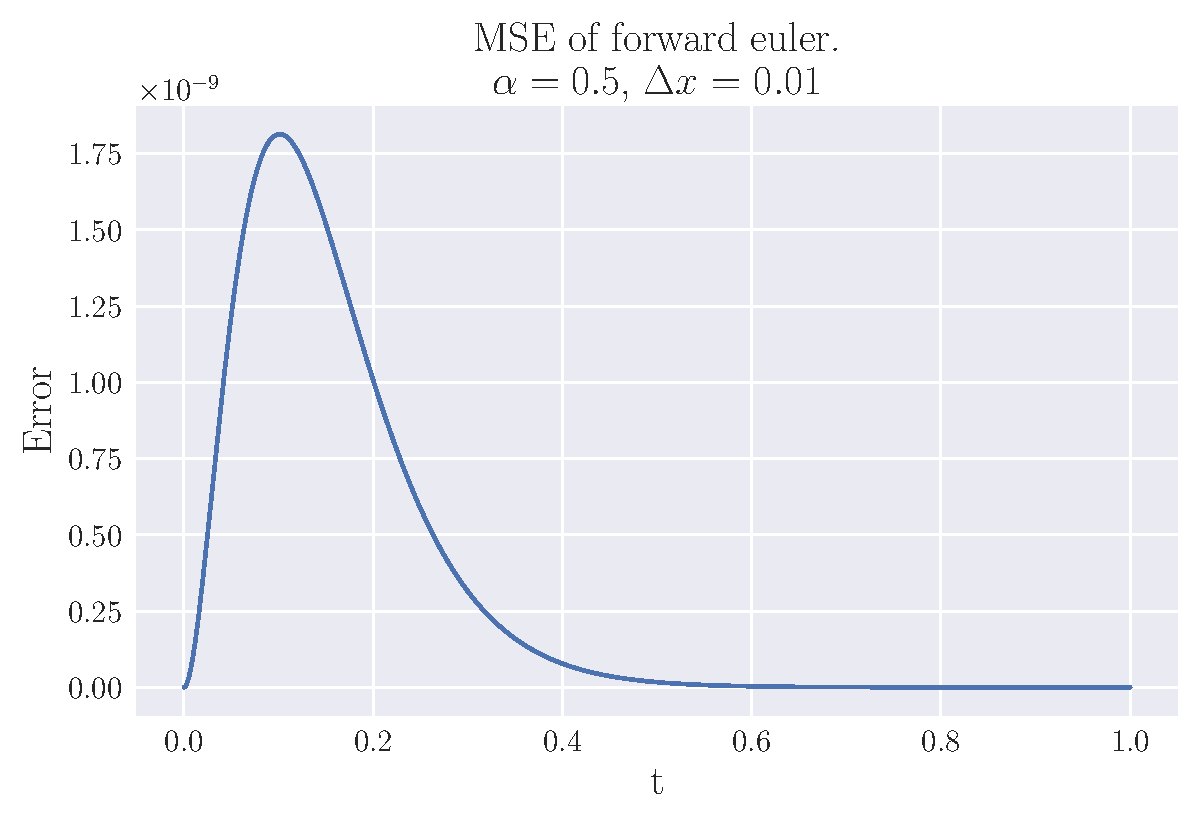
\includegraphics[scale=0.5]{../output/plots/MSE_FE_dx_001.pdf}
	\caption{Mean squared error of approximated solution by forward euler, using $\Delta x=0.01$ and time step $\Delta t$ dictated by the stability criterion \ref{eq:stability}.}
	\label{fig:FE_MSE}
\end{figure}

Figure \ref{fig:NN_MSE} shows the MSE from the neural network with the architecture that provided best results. \textcolor{red}{Sigurd: Legg til MSE plottet her for det beste nettverket.}

Table \ref{tab:MSE_compare} compares the MSE obtained for forward euler and neural network at two selected time steps $t$ and two different spatial steps $\Delta x$. 


\begin{table}[]
	\begin{tabular}{l|ll|ll|}
		\cline{2-5}
		& \multicolumn{2}{l|}{\textbf{$\Delta x=0.1$}}           & \multicolumn{2}{l|}{\textbf{$\Delta x=0.01$}}           \\ \cline{2-5} 
		& \multicolumn{1}{l|}{\textbf{FE}}         & \textbf{NN} & \multicolumn{1}{l|}{\textbf{FE}}          & \textbf{NN} \\ \hline
		\multicolumn{1}{|l|}{\textbf{$t_1=0.1$}} & \multicolumn{1}{l|}{$1.72\cdot 10^{-5}$} &             & \multicolumn{1}{l|}{$1.81\cdot 10^{-9}$}  &             \\ \hline
		\multicolumn{1}{|l|}{\textbf{$t_2=0.5$}} & \multicolumn{1}{l|}{$1.50\cdot 10^{-7}$} &             & \multicolumn{1}{l|}{$1.69\cdot 10^{-11}$} &             \\ \hline
	\end{tabular}
\caption{MSE as function of spatial step $\Delta x$ for two different time levels, for forward euler scheme and neural network. Forward euler is abbreviated as FE and neural network as NN.}
\label{tab:MSE_compare}
\end{table}


\subsection*{Error of Neural Network}

Figure \ref{fig:error_NN_10000} shows the error of the neural network when approximating the solution $u_{\theta}$ to the actual solution $u$ as a function of training iterations. Initially, the error decreases extremely fast - it reduces by a factor of ten for just a couple of iterations, and the approximated solution improves significantly. Afterwards, the error decreases by a much slower rate with some minor fluctuations. Some time after 100 iterations the error is subject to a large jump, but quickly diminishes agains. For later iterations the error slowly converges towards zero, possessing some irregular, minor fluctuations. 

\par \textcolor{red}{PUT THIS IN DISUSSION?:} The reason that the error flucuates instead of decreasing monotonically is that we use the Adam optimizer [\textcolor{red}{https://arxiv.org/abs/1412.6980}]. This is a type of stochastic optimization method, providing more favorable features than traditional stochastic methods. The stochasticity allows the neural network to explore more of the convex parameter space by trying out new, potentially worse solutions. The hope is that, after escaping the local optima, that we find an even better solution at some later stage. The apparent jump in Figure \ref{fig:error_NN_10000} is an example of escaping a local optima at the expense of further exploration. In this case, it does not seem like the new solutions lead to better performance than the previous optima. It eventually converges to zero, which is something the solutions prior to the jump did as well. 

\subsection*{Comparison of error}

\textcolor{red}{IS THIS THE RIGHT WAY TO COMPARE ERROR ??}
 

\section{Discussion}

\subsection*{Performance of Forward Euler}
Figure \ref{fig:FE_MSE} verifies that simulating the forward euler scheme of the diffusion equation with spatial step $\Delta x = 0.01$ yields an excellent correspondance between the numerical and analytical solution. The maximum error is obtained at an early time step, around $\Delta t = 0.1$. For time levels beyond this, the MSE decreases exponentially and eventually converges towards zero. Notice that the error is exactly zero initially, because the numerical scheme has enforced the solution at the initial time step to satisfy the initial condition from the analytical solution.
\par The shape of the plot is in good correspondance with what was initially expected, as elaborated on in Methods. The large initial increase of the MSE is a result of the curved initial solution. The spatial gradients are significant and the approximation with finite differences becomes less accurate.
In the beginning of the diffusion process, for low $t$, the solution changes rather quickly. The forward euler scheme is first order accurate in time, $O(\Delta t)$, and second order accurate in space, $O(\Delta x^2)$, implying that the numerical solution is more sensitive to the temporal evolution than the spatial evolution. Hence, the forward euler scheme will produce larger errors for the initial time levels due to the rapid change in solution \cite{Linge2017}.
\par After time $t=0.1$ the MSE decreases. This can be explained by the discretization parameters $\Delta t$ and $\Delta x$. The magnitude of the gradients are diminished because the solution becomes more linear and less curved. As a result, the solution changes more slowly, allowing the finite difference scheme to approximate the changes more accurately both spatially and temporally. Eventually, the exact solution is approximately constant at zero. In this case, the gradients of the solution are indiscernible and the numerical scheme is able to approximate the solution with machine precision. Figure \ref{fig:FE_MSE} illustrates this by the MSE converging towards zero sufficiently deep into the diffusion process.

\subsection*{Performance of neural network}

\subsection*{Potential for solving differential equations}
The forward euler method and neural networks are two quite different methods for solving differential equations. The former relies on discretization of the derivative to arrive at an explicit recursive set of equations to solve for each time step. The latter uses the residual error from the approximation as a basis for backpropagation to update weights and biases to improve the approximation to the actual solution. Figure \ref{fig:error_NN_40000} visualizes how bad the approximated solution of the initial run of the neural network is. Just after a few iterations though, the error decreases tremendously and goes below 0.083 (which is the total error obtained from forward euler) after around 100 iterations. After this, the total error fluctuates mildly but eventually converges towards zero.
 
\par The forward euler method clearly has an advantage in its simple recursive formula and fast computation time. The proposed solution is calculated within a few milliseconds, with a total error of only 0.083. On the other hand, it is limited by a stability requirement in order to produce realistic results. This effectively puts a restriction on applicable mesh resolutions.

\par A notable drawback of the neural network is the demanding training process. To compute an approximated solution of \ref{eq:diffusion_equation_1D} requires calculating gradients and accumulating chained derivatives backwards through the hidden layers. This is a significantly larger computational effort than calculating the simple recursive formula of the forward euler scheme. As a result, the neural network suffers from a large computational runtime. Still, if training sufficiently long, the neural network will produce a better solution than forward euler and eventually yield a near perfect approximation to the exact solution. 

\par The forward euler scheme has proven to obtain good accuracy on the numerical solution. However, forward euler has an inherent disadvantage in that it is conditionally unstable with stability criteria given by \ref{eq:stability}. In general it means that the forward euler scheme is not a stable method for solving differential equations as it requires that we carefully assign the mesh discretization steps. Neural networks are not limited to any kind of discretization. Neural networks benefit from good convergence properties. That is, given enough time to train it is able to approximate the actual solution of a differential equation with an error of approximately zero. Moreover, the neural network model \ref{eq:NN_model} has the additional flexibility in that the function $f$ can be tweaked to give a better initial guess of the solution. 
\par Overall, the method of choice for solving differential equations is a tradeoff between the accuracy of the approximated solution and the computational runtime. Forward euler is definitely the desired method if we want a quick representation of the solution. If the importance is how precise the representation is, a neural network is a better choice.

\textcolor{red}{Det meste av diskusjonen over kan beholdes da det gjelder generelt, men de faktiske tallene nevnt maa oppdateres med resultatene fra MSE.}


\section{Conclusion}

\bibliographystyle{plain}
\bibliography{refs}
\end{document}

